%%%%%%%%%%%%%%%%%%%%%%%%%%%%%%%%%%%%%%%%%
% Short Sectioned Assignment LaTeX Template Version 1.0 (5/5/12)
% This template has been downloaded from: http://www.LaTeXTemplates.com
% Original author:  Frits Wenneker (http://www.howtotex.com)
% License: CC BY-NC-SA 3.0 (http://creativecommons.org/licenses/by-nc-sa/3.0/)
%%%%%%%%%%%%%%%%%%%%%%%%%%%%%%%%%%%%%%%%%

%----------------------------------------------------------------------------------------
%	PACKAGES AND OTHER DOCUMENT CONFIGURATIONS
%----------------------------------------------------------------------------------------

\documentclass[paper=a4, fontsize=11pt]{scrartcl} % A4 paper and 11pt font size

% ---- Entrada y salida de texto -----

\usepackage[T1]{fontenc} % Use 8-bit encoding that has 256 glyphs
\usepackage[utf8]{inputenc}

% ---- Idioma --------

\usepackage[spanish, es-tabla]{babel} % Selecciona el español para palabras introducidas automáticamente, p.ej. "septiembre" en la fecha y especifica que se use la palabra Tabla en vez de Cuadro

% ---- Otros paquetes ----

\usepackage{amsmath,amsfonts,amsthm} % Math packages
\usepackage{graphics,graphicx, floatrow} %para incluir imágenes y notas en las imágenes
\usepackage{graphics,graphicx, float} %para incluir imágenes y colocarlas
\usepackage{hyperref} % url in references
\usepackage{listings}
\usepackage{color}
\definecolor{grey}{gray}{0.9}

% Para hacer tablas comlejas
\usepackage{multirow}
\usepackage{threeparttable}

\usepackage{fancyhdr} % Custom headers and footers
\pagestyle{fancyplain} % Makes all pages in the document conform to the custom headers and footers
\fancyhead{} % No page header - if you want one, create it in the same way as the footers below
\fancyfoot[L]{} % Empty left footer
\fancyfoot[C]{} % Empty center footer
\fancyfoot[R]{\thepage} % Page numbering for right footer
\renewcommand{\headrulewidth}{0pt} % Remove header underlines
\renewcommand{\footrulewidth}{0pt} % Remove footer underlines
\setlength{\headheight}{13.6pt} % Customize the height of the header

\numberwithin{equation}{section} % Number equations within sections (i.e. 1.1, 1.2, 2.1, 2.2 instead of 1, 2, 3, 4)
\numberwithin{figure}{section} % Number figures within sections (i.e. 1.1, 1.2, 2.1, 2.2 instead of 1, 2, 3, 4)
\numberwithin{table}{section} % Number tables within sections (i.e. 1.1, 1.2, 2.1, 2.2 instead of 1, 2, 3, 4)

\setlength\parindent{0pt} % Removes all indentation from paragraphs - comment this line for an assignment with lots of text

\newcommand{\horrule}[1]{\rule{\linewidth}{#1}} % Create horizontal rule command with 1 argument of height

\usepackage{textcomp}
\usepackage{hyperref}

%----------------------------------------------------------------------------------------
%	DATOS
%----------------------------------------------------------------------------------------

\newcommand{\myName}{Francisco Javier Bolívar Lupiáñez}
\newcommand{\myMail}{fblupi@correo.ugr.es}
\newcommand{\myDNI}{75926571-Y}
\newcommand{\myDegree}{Máster en Ingeniería Informática}
\newcommand{\myFaculty}{E. T. S. de Ingenierías Informática y de Telecomunicación}
\newcommand{\myDepartment}{Ciencias de la Computación e Inteligencia Artificial}
\newcommand{\myUniversity}{\protect{Universidad de Granada}}
\newcommand{\myLocation}{Granada}
\newcommand{\myTime}{\today}
\newcommand{\myTitle}{Práctica 2}
\newcommand{\mySubtitle}{Caso Práctico de Análisis y Evaluación de Redes en Twitter}
\newcommand{\mySubject}{Gestión de Información en la Web}
\newcommand{\myYear}{2016-2017}

%----------------------------------------------------------------------------------------
%	PORTADA
%----------------------------------------------------------------------------------------


\title{	
	\normalfont \normalsize 
	\textsc{\textbf{\mySubject \space (\myYear)} \\ \myDepartment} \\[20pt] % Your university, school and/or department name(s)
	\textsc{\myDegree \\[10pt] \myFaculty \\ \myUniversity} \\[25pt]
	\horrule{0.5pt} \\[0.4cm] % Thin top horizontal rule
	\huge \myTitle: \mySubtitle \\ % The assignment title
	\horrule{2pt} \\[0.5cm] % Thick bottom horizontal rule
	\normalfont \normalsize
}

\author{
	\myName \\
	\small \texttt{\myMail} \\
	\small \myDNI \\
}

\date{\myTime} % Incluye la fecha actual
%----------------------------------------------------------------------------------------
%	INDICE
%----------------------------------------------------------------------------------------

\begin{document}
	
\definecolor{light-gray}{gray}{0.95}
	
\lstset {
	basicstyle=\scriptsize,
	frame=single,
	backgroundcolor=\color{grey}
}
	
\setcounter{page}{0}

\maketitle % Muestra el Título
\thispagestyle{empty}

\newpage %inserta un salto de página

\tableofcontents % para generar el índice de contenidos

\newpage %inserta un salto de página

\listoffigures

\listoftables

\newpage

%----------------------------------------------------------------------------------------
%	DOCUMENTO
%----------------------------------------------------------------------------------------

\section{Introducción}
\label{sec:intro}

El medio social que he escogido ha sido Twitter ya que se nos ha proporcionado una herramienta para su fácil extracción de datos (NodeXL) sin tener que perder tiempo programando llamadas a la API de Twitter.
\\ \\
La elección del tema fue más complicado, pues sabía que lo mejor era utilizar un tema que conociese y no cualquier \textit{trending topic} que viese un día. Por ello, tras estar varios días extrayendo redes de distintas temáticas, me decidí por la red obtenida tras el primer Gran Premio de Fórmula 1 de la temporada 2017/2018 celebrado en Australia con el \textit{hash tag} oficial \#AusGP.
\\ \\
La Fórmula 1 tiene un gran número de seguidores alrededor de todo el mundo. Hay muchos que durante una carrera mencionan a cualquier piloto o escudería, por lo que acaban mencionando al que hace cosas más destacables durante la carrera, y otros, más fanáticos, que mencionan solo al piloto de su país o escudería preferida. Por lo tanto, mi pregunta es: ¿Qué tipo de aficionado es el mayoritario, el neutral que menciona a más de un piloto o escudería o el fanático que solo menciona a un piloto o escudería? Al mismo tiempo, se podrán ver quiénes fueron los usuarios más mencionados tras el Gran Premio, ¿coincidirá con los protagonistas de la carrera?
\\ \\
Para la extracción de datos se ha utilizado, como se ha mencionado anteriormente, NodeXL en su versión gratuita limitada, por tanto, nos encontramos con una limitación de un máximo de 2000 tuits cada vez que extrajésemos datos. Para lidiar con ello y poder obtener una red más grande se extrajeron datos de un periodo de tiempo a otro, obteniendo los tuits que transcurrieron durante las siguiente franjas horarias:

\begin{itemize}
	\item 9:33 - 9:38 (Recién terminada la carrera)
	\item 13:59 - 14:33 (Recién terminada la carrera en su segunda emisión en horario europeo)
	\item 15:30 - 17:09 (Tras los informativos televisivos)
\end{itemize}

La primera conclusión que podemos extraer de aquí es que el tiempo de actividad es mucho mayor durante la carrera en directo que durante la carrera en diferido (pese a ser una hora bastante mala para los aficionados europeos pues tuvieron que madrugar un domingo para poder verla).

\section{Estructura de la red}

En la red extraída desde NodeXL los nodos son los usuarios (con información adicional como su número de seguidores, de usuarios que siguen, tuits o tuits marcacdos como favoritos) y las aristas son la interacción entre usuarios (mención, respuesta o retuit), por tanto se trata de una red dirigida.
\\ \\
La red original consta de 4601 nodos y 6698 aristas. Aplicando un primer filtro de componente gigante para deshacerse de grupos pequeños que no interaccionan con el grupo más grande, pasamos a 3476 nodos y 5703 aristas (el 75,55\% y 85,14\% respectivamente con respecto a la red social original).
\\ \\
A continuación se ha aplicado un filtro de \textit{k-core} con grado 3 para seguir simplificándola pues seguía siendo todavía demasiado grande y difícil de visualizar. Aplicando este filtro pasamos a 532 nodos y 1783 aristas.

\section{Valores de medidas de análisis}
\label{sec:medidas}

\subsection{Red original}

\begin{table}[H]
	\centering
	\caption{Valores de las medidas de análisis de la red original}
	\label{tab:medidas-original}
	\begin{tabular}{| l | l |}
		\hline
		Medida                						& Valor          \\ 
		\hline
		$N$                   						& 4601           \\
		$L$                   						& 6704           \\
		$D$                   						& 0,0003         \\
		$k$                   						& 1,457          \\
		$d_{max}$             						& 4              \\
		$d$                   						& 1,179          \\
		$d_{aleatoria} (\frac{log(N)}{log(k)})$		& 22,408         \\
		$C$                   						& 0,079          \\
		$C_{aleatoria} (\frac{k}{N})$       		& 0,0003         \\
		Componentes conexas   						& 432            \\ 
		$N_{gigante}$         						& 3476 (75,55\%) \\ 
		$L_{gigante}$         						& 5703 (85,14\%) \\ 
		\hline
	\end{tabular}
\end{table}

La densidad de la red original es muy pequeña. Vemos que hay casi el mismo número de nodos que de enlaces, ya que muchos usuarios solo mencionarían a un usuario. La mayoría a la cuenta oficial de F1 (\textit{@f1}) pero muchos otros a Ferrari (\textit{@scuderiaferrari}) ya que Sebastian Vettel (el cual no tiene cuenta oficial de Twitter) fue quien, ante todo pronóstico, ganó la carrera.
\\ \\
La distancia media de un nodo a otro es muy pequeña lo cual es lógico al haber nodos que están conectados con un enorme número de usuarios. Además, el diámetro es de tan solo 4, por lo que, como muchos en 4 pasos, se podría pasar de un nodo a cualquier otro.
\\ \\
El coeficiente de clustering medio es muy bajo y el de para una red aleatoria más bajo todavía. Y es que como podemos ver hay hasta 432 componentes conexas lo cual puede explicar este valor tan bajo. En muchos casos es debido a usuarios que responden a otros usando el \textit{hash tag} sin mencionar a ningún otro usuario.

\subsection{Red filtrada}

\begin{table}[H]
	\centering
	\caption{Valores de las medidas de análisis de la red filtrada}
	\label{tab:medidas-filtrada}
	\begin{tabular}{| l | l |}
		\hline
		Medida                						& Valor        \\ 
		\hline
		$N$                   						& 532          \\
		$L$                   						& 1783         \\
		$D$                 						& 0,006        \\
		$k$                  						& 3,352        \\
		$d_{max}$             						& 4            \\
		$d$                   						& 1,189        \\
		$d_{aleatoria} (\frac{log(N)}{log(k)})$		& 5,189        \\
		$C$                   						& 0,131        \\
		$C_{aleatoria} (\frac{k}{N})$       		& 0,006        \\ 
		Componentes conexas   						& 1            \\ 
		$N_{gigante}$         						& 532 (100\%)  \\ 
		$L_{gigante}$         						& 1783 (100\%) \\ 
		\hline
	\end{tabular}
\end{table}

La densidad sigue siendo pequeña pero es bastante mayor que la de la red original (20 veces mayor).
\\ \\
La distancia apenas varía de la red original a la filtrada, aumenta tan solo en 0,01, mientras que el diámetro se mantiene en 4.
\\ \\
El coeficiente de \textit{clustering} sigue siendo bastante pequeño, lo cual puede hacer difícil la detección de comunidades para un número de comunidades pequeña.
\\ \\
En este caso, al haberse filtrado la red previamente usando la componente gigante, el número de componentes conexas es 1, como no podría ser de otra manera.

\section{Propiedades de la red}

A continuación se describirán propiedades de la red ya filtrada, que será sobre la que se haga la detección de comunidades y visualización.

\subsection{Distribución de grados}

\begin{figure}[H]
	\centering
	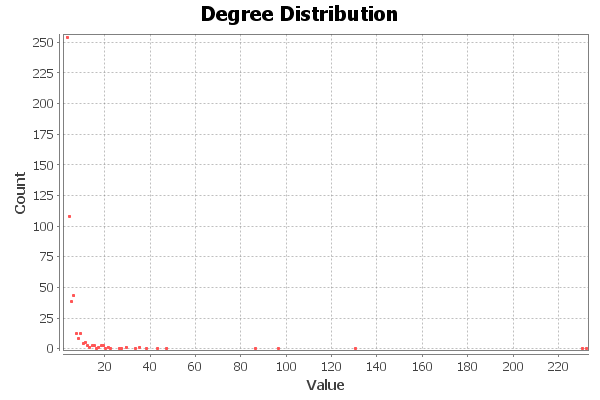
\includegraphics[width=12cm]{img/degree-distribution-filtered}
	\caption{Distribución de grados para la red filtrada}
	\label{fig:degree-distribution-filtered}
\end{figure}

\begin{figure}[H]
	\centering
	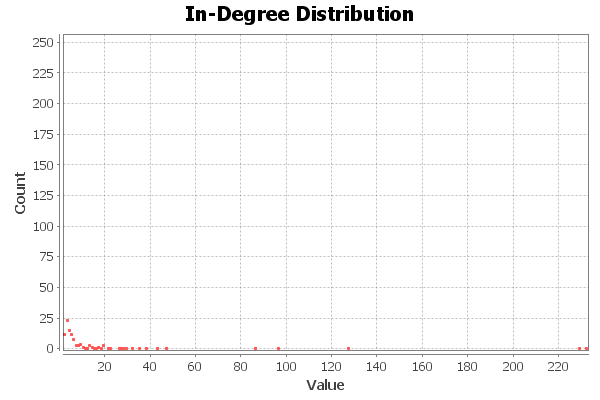
\includegraphics[width=12cm]{img/in-degree-distribution-filtered}
	\caption{Distribución de grados de entrada para la red filtrada}
	\label{fig:in-degree-distribution-filtered}
\end{figure}

\begin{figure}[H]
	\centering
	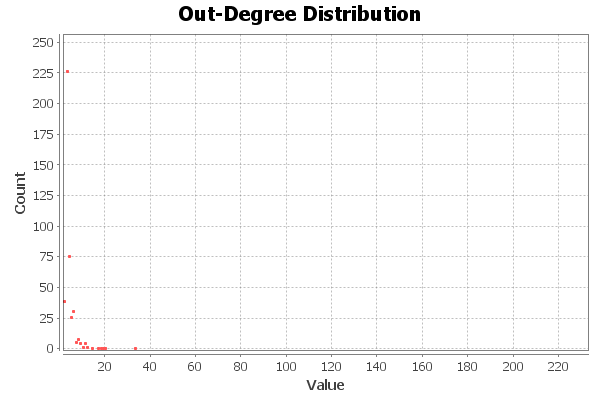
\includegraphics[width=12cm]{img/out-degree-distribution-filtered}
	\caption{Distribución de grados de salida para la red filtrada}
	\label{fig:out-degree-distribution-filtered}
\end{figure}

Se puede observar como se cumple la ley de la potencia: $ P(k) \sim k^{-\gamma} $ y es que la mayoría de los nodos tienen pocos enlaces pero hay unos cuantos \textit{hubs} que tienen muchos, y posteriormente, al visualizarlo se verá una forma de estrella alrededor de estos. Por tanto podríamos decir que la red es libre de escala.

\subsection{Distribución de distancias}

\begin{figure}[H]
	\centering
	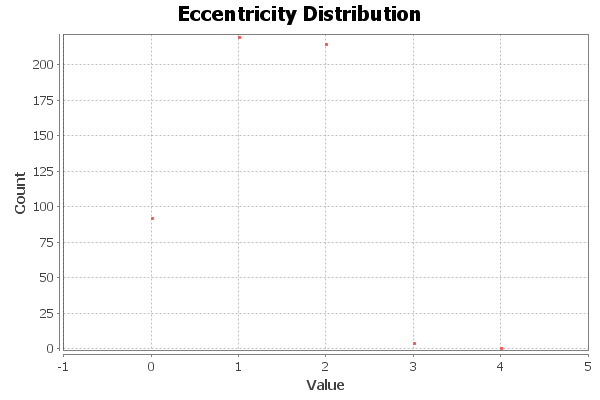
\includegraphics[width=12cm]{img/eccentricity-distribution-filtered}
	\caption{Distribución de excentricidad para la red filtrada}
	\label{fig:eccentricity-distribution-filtered}
\end{figure}

En este gráfico (Figura \ref{fig:eccentricity-distribution-filtered}) vemos que hay bastantes nodos con distancia 0, esto es porque en el grafo hay nodos con grado de salida 0 y al ser una red dirigida es imposible llegar a ellos.
\\ \\
Recordamos, el diámetro de la red era 4 y la distancia media 1,189. En la distribución vemos como a mayor sea el valor de distancia, menor es el número de nodos. Esto es consecuencia de cumplir la propiedad de mundo pequeño. Además si calculamos la distancia aleatoria como $ \dfrac{log(N)}{log(log(N))} $ el resultado es 3,417 aún mayor que la distancia real. Por tanto estamos ante un mundo ultra pequeño.

\subsection{Distribución de coeficientes de clustering}

\begin{figure}[H]
	\centering
	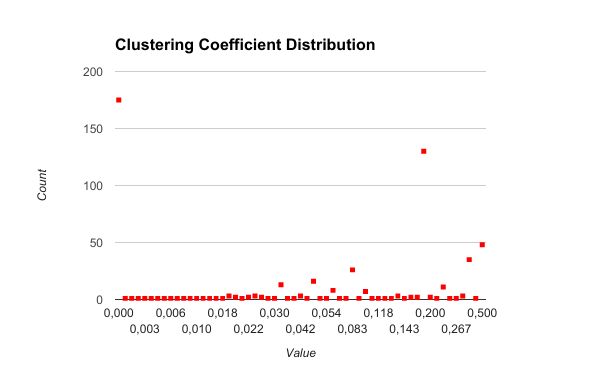
\includegraphics[width=12cm]{img/clustering-coefficient-distribution-filtered}
	\caption{Distribución de coeficiente de clustering para la red filtrada}
	\label{fig:clustering-coefficient-distribution-filtered}
\end{figure}

El coeficiente de clustering de la red social es bastante bajo, de tan solo 0,131.
\\ \\
Se ve también que los nodos con mayor coeficiente de clustering coinciden con los menos importantes que se verán en la Sección \ref{sec:hubs}. Esto es consecuencia de la jerarquía de redes.

\section{Medidas de centralidad para nodos principales}
\label{sec:hubs}

En esta sección se va a intentar detectar a los actores principales dentro de la red social utilizando varias medidas: grado, intermediación, cercanía y vector propio.
\\ \\
Se presentarán en tablas con los 10 primeros actores y el valor que tienen para cada medida.

\begin{table}[H]
	\centering
	\caption{Actores principales según el grado}
	\label{tab:actores-principales-grado}
	\begin{tabular}{| l | l l l |}
		\hline
		\# & \textit{degree}       & \textit{in-degree}     & \textit{out-degree}   \\
		\hline
		1  & [232] scuderiaferrari & [232] scuderiaferrari  & [33] cheekycorini     \\
		2  & [230] f1              & [229] f1               & [20] stevestevens47   \\
		3  & [130] mercedesamgf1   & [127] mercedesamgf1    & [19] eko\_sap56963457 \\
		4  & [96] valtteribottas   & [96] valtteribottas    & [18] alejand20099936  \\
		5  & [86] lewishamilton    & [86] lewishamilton     & [17] americoscatena   \\
		6  & [47] ausgrandprix     & [47] ausgrandprix      & [14] juanbernalm      \\
		7  & [43] sebvettelnews    & [43] sebvettelnews     & [12] fishtrenado      \\
		8  & [38] oconesteban      & [38] oconesteban       & [12] mireillebrigit   \\
		9  & [35] skysportf1hd     & [35] forceindiaf1      & [11] f1\_images       \\
		10 & [35] forceindiaf1     & [32] skysportf1hd      & [11] wakeupmob        \\
		\hline
	\end{tabular}
\end{table}

\begin{table}[H]
	\centering
	\caption{Actores principales según la intermediación y cercanía.}
	\label{tab:actores-principales-intermediacion-cercania}
	\begin{tabular}{| l | l l |}
		\hline
		\# & \textit{betweeness centrality} & \textit{closness centrality} \\
		\hline 
		1  & [142] mercedesamgf1            & [1] mercedesamgf1            \\
		2  & [73,833] f1                    & [1] f1                       \\
		3  & [73,5] skysportf1hd            & [1] skysportf1hd             \\
		4  & [13] motorlat                  & [1] motorlat                 \\
		5  & [9] c4f1                       & [1] c4f1                     \\
		6  & [8] saetta\_mcqueen            & [1] alayzell20297            \\
		7  & [7] maui27575                  & [1] f1writers                \\
		8  & [6,333] graftechweb            & [1] alexs1man                \\
		9  & [6] motorsport\_it             & [1] dan\_rigsby              \\
		10 & [6] guilialabo                 & [1] vettel\_formel1          \\
		\hline
	\end{tabular}
\end{table}

\begin{table}[H]
	\centering
	\caption{Actores principales según el vector propio y \textit{pagerank}}
	\label{tab:actores-principales-vector-propio}
	\begin{tabular}{| l | l l |}
		\hline
		\# & \textit{eigen centrality} & \textit{pagerank}       \\
		\hline 
		1  & [1] scuderiaferrari       & [0,084] scuderiaferrari \\
		2  & [0,723] f1                & [0,043] f1              \\
		3  & [0,542] mercedesamgf1     & [0,030] mercedesamgf1   \\
		4  & [0,451] valteribottas     & [0,028] redbullracing   \\
		5  & [0,421] lewishamilton     & [0,025] valtteribottas  \\
		6  & [0,153] oconesteban       & [0,024] lewishamilton   \\
		7  & [0,140] ausgrandprix      & [0,022] gianludale27    \\
		8  & [0,130] sebvettelnews     & [0,020] enricotornello  \\
		9  & [0,130] danielricciardo   & [0,019] motorsport      \\
		10 & [0,119] redbullracing     & [0,014] a3formula1      \\
		\hline
	\end{tabular}
\end{table}

En las Tablas \ref{tab:actores-principales-grado} y \ref{tab:actores-principales-intermediacion-cercania} podemos ver como dos medidas no nos van a servir para detectar a nuestros actores principales:

\begin{itemize}
	\item \textit{out-degree}: Representa a los usuarios que más veces han interaccionado. Pueden haber mencionado muchas veces, pero lo que buscamos son los mencionados, no los que mencionan.
	\item \textit{closness centrality}: Los 220 primeros nodos tienen valor 1 por lo que no es un dato que nos sirva para detectar a los actores principales.
\end{itemize}

Además el grado (\textit{degree}) y el grado de entrada (\textit{in-degree}) se parecen mucho. Vemos que, excepto \textit{skysportf1hd} (cuenta oficial de F1 de un canal televisivo), en el resto de los dos primeros coinciden. Esto es porque han sido mencionados pero no han mencionado a nadie (o no se ha recogido el tuit por haberse generado entre las horas que se recogió la información).
\\ \\
No obstante, antes que considerar el grado para medir la centralidad, sería más apropiado utilizar el vector propio (\textit{eigen centrality}) o el \textit{pagerank} (Tabla \ref{tab:actores-principales-vector-propio}) pues agrega otra información importante y es que pondera las conexiones según lo central que sea el nodo con el que se conecta. De esta forma se mediría la calidad y no la cantidad de enlaces.

\section{Comunidades}

Se ha utilizado Gephi para detectar comunidades dando una resolución de 1,5 y obteniendo 9 comunidades y un coeficiente de 0,412, el cual supera la barrera de 0,3 para considerarlo aceptable.
\\ \\
Para diferenciar los grupos he buscado las distintas cuentas de escuderías y pilotos:

\begin{itemize}
	\item Escudería Mercedes:
	\begin{itemize}
		\item \textit{@mercedesamgf1}: 2
		\item \textit{@lewishamilton}: 2
		\item \textit{@valtteribottas}: 2
	\end{itemize}

	\item Escudería Ferrari:
	\begin{itemize}
		\item \textit{@scuderiaferrari}: 3
	\end{itemize}

	\item Escudería Red Bull:
	\begin{itemize}
		\item \textit{@redbullracing}: 4
		\item \textit{@danielricciardo}: 4
		\item \textit{@max33verstappen}: 4
	\end{itemize}
	
	\item Escudería Force India:
	\begin{itemize}
		\item \textit{@forceindiaf1}: 5
		\item \textit{@schecoperez}: 7
		\item \textit{@oconesteban}: 5
		\item \textit{@thevijaymallya}: 5
	\end{itemize}

	\item Escudería Williams:
	\begin{itemize}
		\item \textit{@williamsracing}: 5
		\item \textit{@massafelipe19}: 5
		\item \textit{@lance\_stroll}: 0
	\end{itemize}

	\item Escudería McLaren:
	\begin{itemize}
		\item \textit{@mclarenf1}: 0
		\item \textit{@alo\_oficial}: 2
		\item \textit{@svandoorne}: 0
	\end{itemize}

	\item Escudería Toro Rosso:
	\begin{itemize}
		\item \textit{@tororossospy}: 5
		\item \textit{@carlossainz55}: 5
		\item \textit{@kvyatofficial}: 5
	\end{itemize}

	\item Escudería Haas:
	\begin{itemize}
		\item \textit{@haasf1team}: 5
		\item \textit{@rgrosjean}: 0
		\item \textit{@kevinmagnussen}: 0
	\end{itemize}

	\item Escudería Renault:
	\begin{itemize}
		\item \textit{@renaultsportf1}: 5
		\item \textit{@hulkhulkenberg}: 5
		\item \textit{@jolyonpalmer}: 0
	\end{itemize}

	\item Escudería Sauber:
	\begin{itemize}
		\item \textit{@sauberf1team}: 5
		\item \textit{@ericsson\_marcus}: 5
		\item \textit{@anto\_giovinazzi}: 5
	\end{itemize}
\end{itemize} 

Se ve que las tres principales escuderías están en tres comunidades distintas (Mercedes la 2, Ferrari la 3 y Red Bull la 4) mientras que el resto de escuderías se encuentran mayoritariamente en la misma comunidad (la 5). Con algunas excepciones entre las que se pueden destacar a:

\begin{itemize}
	\item Fernando Alonso: que se encuentra en la misma comunidad que Mercedes, posiblemente porque en verano se rumoreó que cambiaría a este equipo donde podría optar a volver a ser campeón del mundo y tras problemas en su coche actual tuvo que abandonar la carrera.
	\item Sergio ``Checo'' Pérez: Único piloto mexicano de la plantilla. Los mexicanos tienen fama de ser muy fanáticos y se encuentra en un grupo independiente con usuarios mayoritariamente mexicanos (Figura \ref{fig:comunidad-perez}).
\end{itemize}
 
\begin{figure}[H]
	\centering
	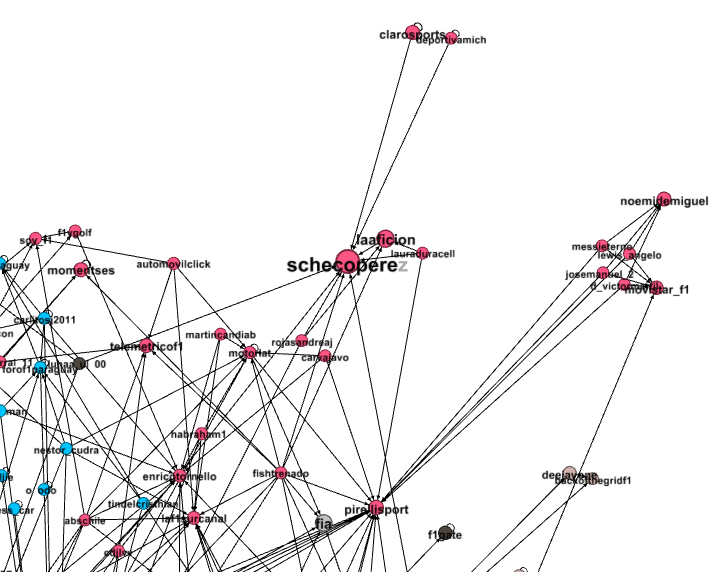
\includegraphics[width=14cm]{img/comunidad-perez}
	\caption{Comunidad alrededor del piloto mexicano Checo Pérez}
	\label{fig:comunidad-perez}
\end{figure}

\section{Visualización}

\begin{figure}[H]
	\centering
	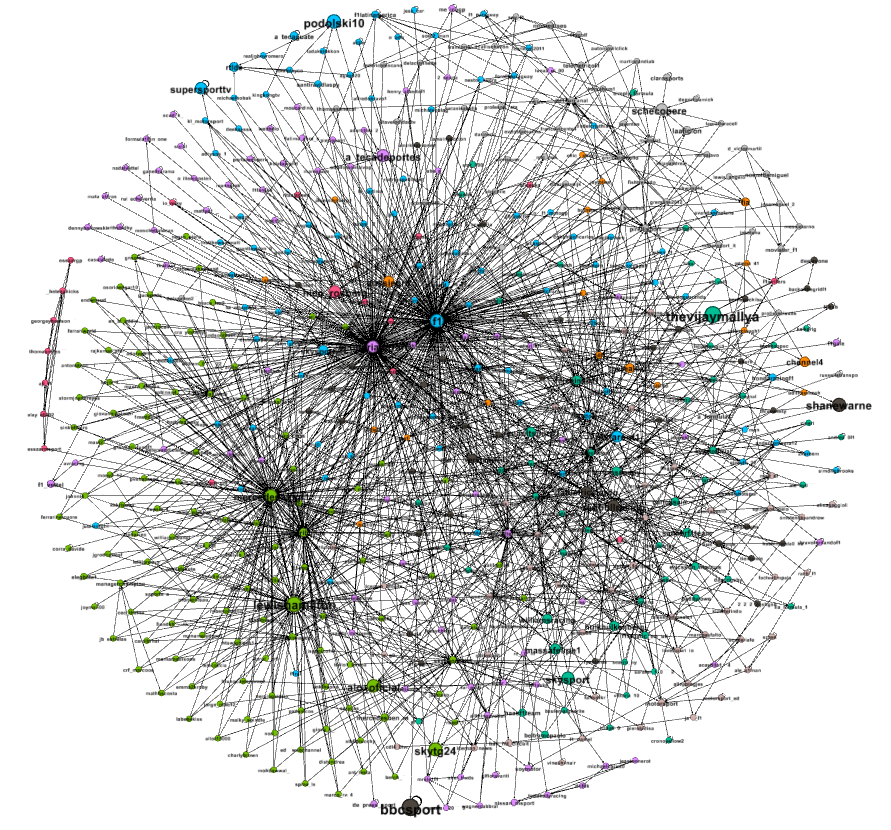
\includegraphics[width=14cm]{img/fruchterman-reingold}
	\caption{Visualización utilizando el algoritmo de Fruchterman Reingold}
	\label{fig:fruchterman-reingold}
\end{figure}

Se han probado los dos algoritmos principales para visualizar las redes (de distribución guiados por fuerzas), en primer lugar el de Fruchterman Reingold usando el número de seguidores para el tamaño del nodo y la comunidad a la que pertenece para el color (Figura \ref{fig:fruchterman-reingold}).
	
\begin{figure}[H]
	\centering
	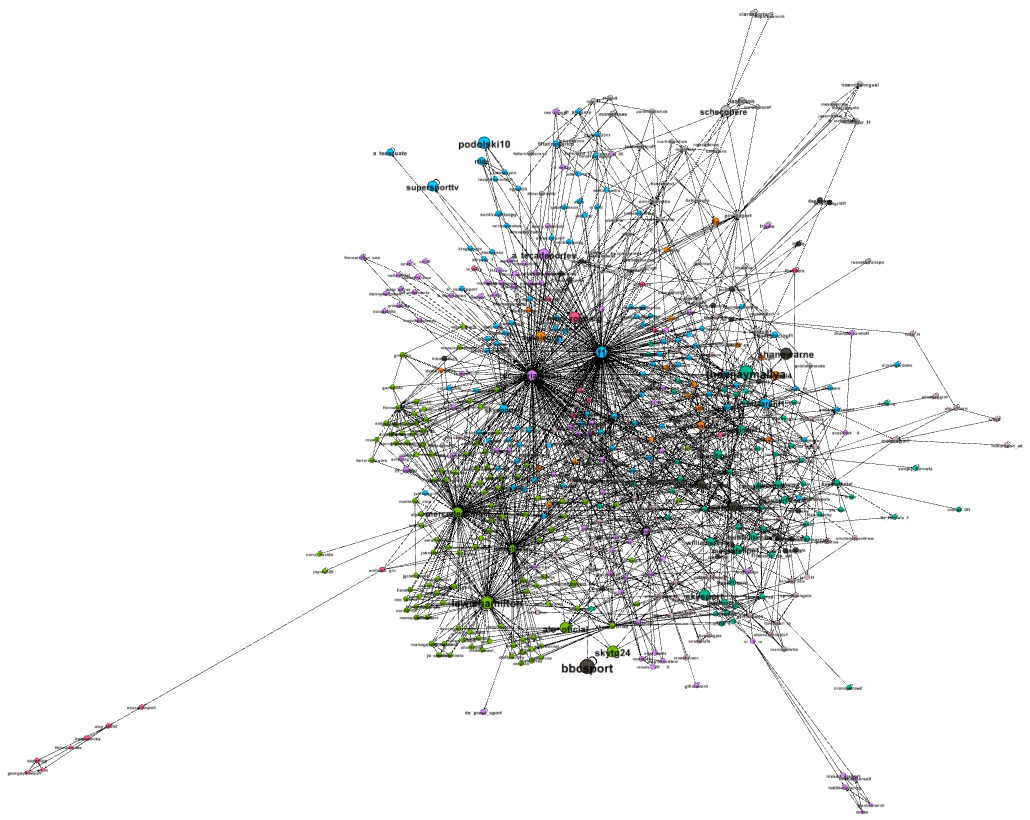
\includegraphics[width=14cm]{img/kamada-kawai}
	\caption{Visualización utilizando el algoritmo de Kamada Kawai}
	\label{fig:kamada-kawai}
\end{figure}

También se ha probado el de Kamada Kawai (\textit{Force Atlas 2} en Gephi) usando el número de seguidores para el tamaño del nodo y la comunidad a la que pertenece para el color (Figura \ref{fig:kamada-kawai}).
\\ \\
Viendo sendas visualizaciones, me parece que aporta más la segunda. Separa muy bien dos comunidades que se alejan bastante del núcleo y dentro de éste la mayoría de los nodos de una misma comunidad están en el centro, excepto los más centrales donde se mezclan de varias comunidades (tal vez porque podrían pertenecer perfectamente a cualquiera).

\begin{figure}[H]
	\centering
	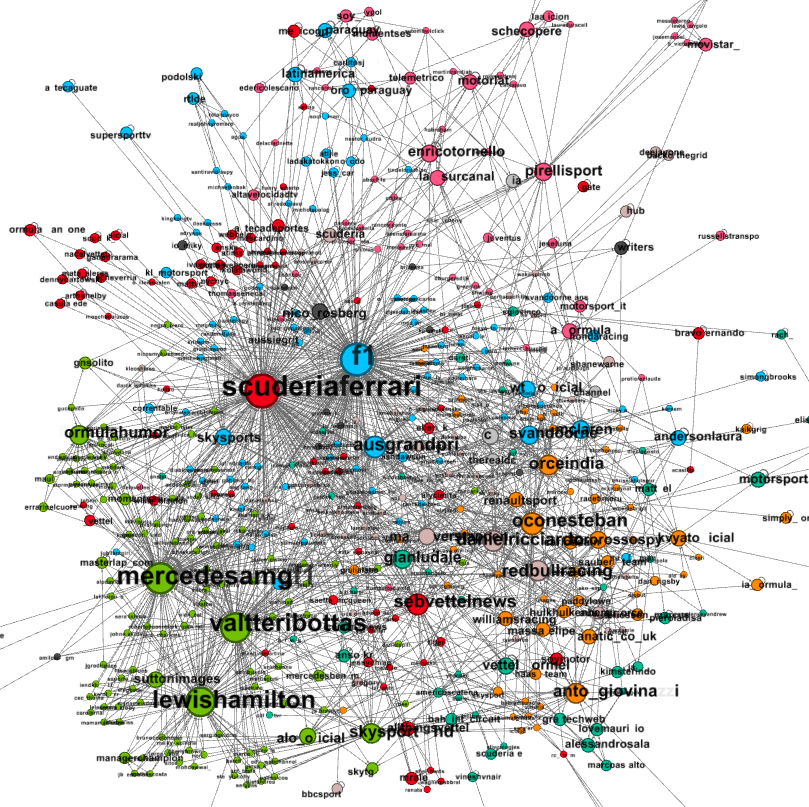
\includegraphics[width=14cm]{img/eigenvector}
	\caption{Visualización utilizando el algoritmo de Kamada Kawai usando el \textit{eigenvector} para colorear los nodos}
	\label{fig:eigenvector}
\end{figure}

Para ver más claramente cuáles son los actores principales (en la sección \ref{sec:hubs} observamos que lo mejor era usar el vector propio), y tras ya haber analizado las comunidades, se va a pasar a cambiar el tamaño para que muestre el vector propio (Figura \ref{fig:eigenvector}) en lugar del número de seguidores.
\\ \\
Los actores principales son:

\begin{itemize}
	\item \textit{@f1}: La cuenta oficial de la Fórmula 1. Lo cuál era de esperar. Además es mencionada por todas las comunidades que se han detectado (Figura \ref{fig:f1-mentions}).
\end{itemize}

\begin{figure}[H]
	\centering
	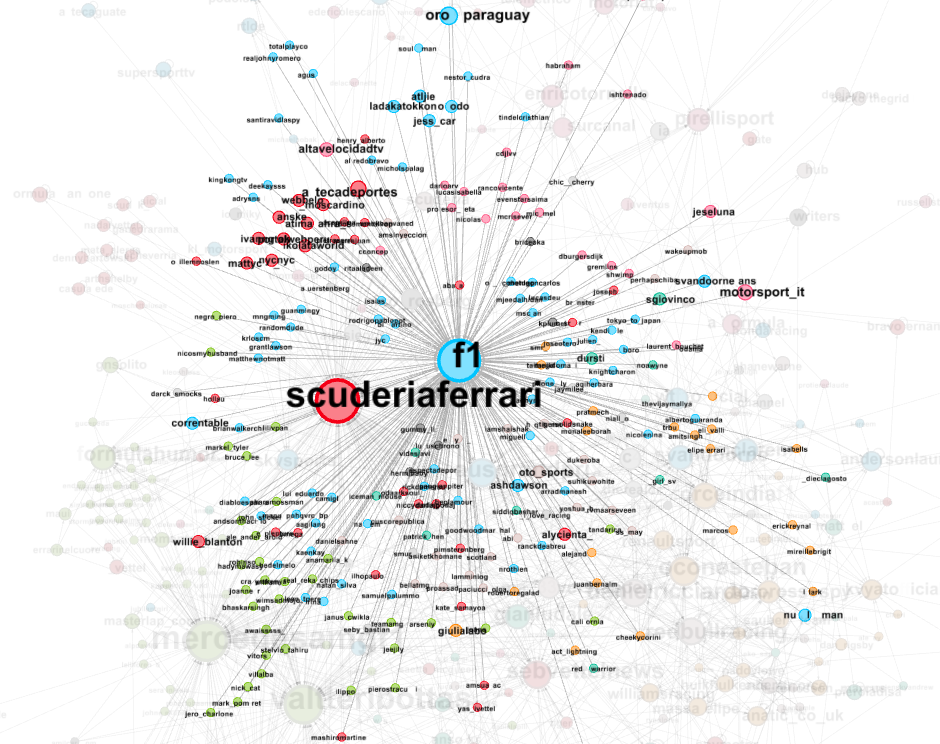
\includegraphics[width=12cm]{img/f1-mentions}
	\caption{Usuarios que mencionan a la cuenta @f1}
	\label{fig:f1-mentions}
\end{figure}

\begin{itemize}
	\item \textit{@scuderiaferrari}: La escudería que ganó la carrera, mencionada por todos los medios de noticias y muchísimos aficionados (además de los que ya tiene). También es mencionada por todas las comunidades detectadas (Figura \ref{fig:scuderiaferrari-mentions}).
\end{itemize}

\begin{figure}[H]
	\centering
	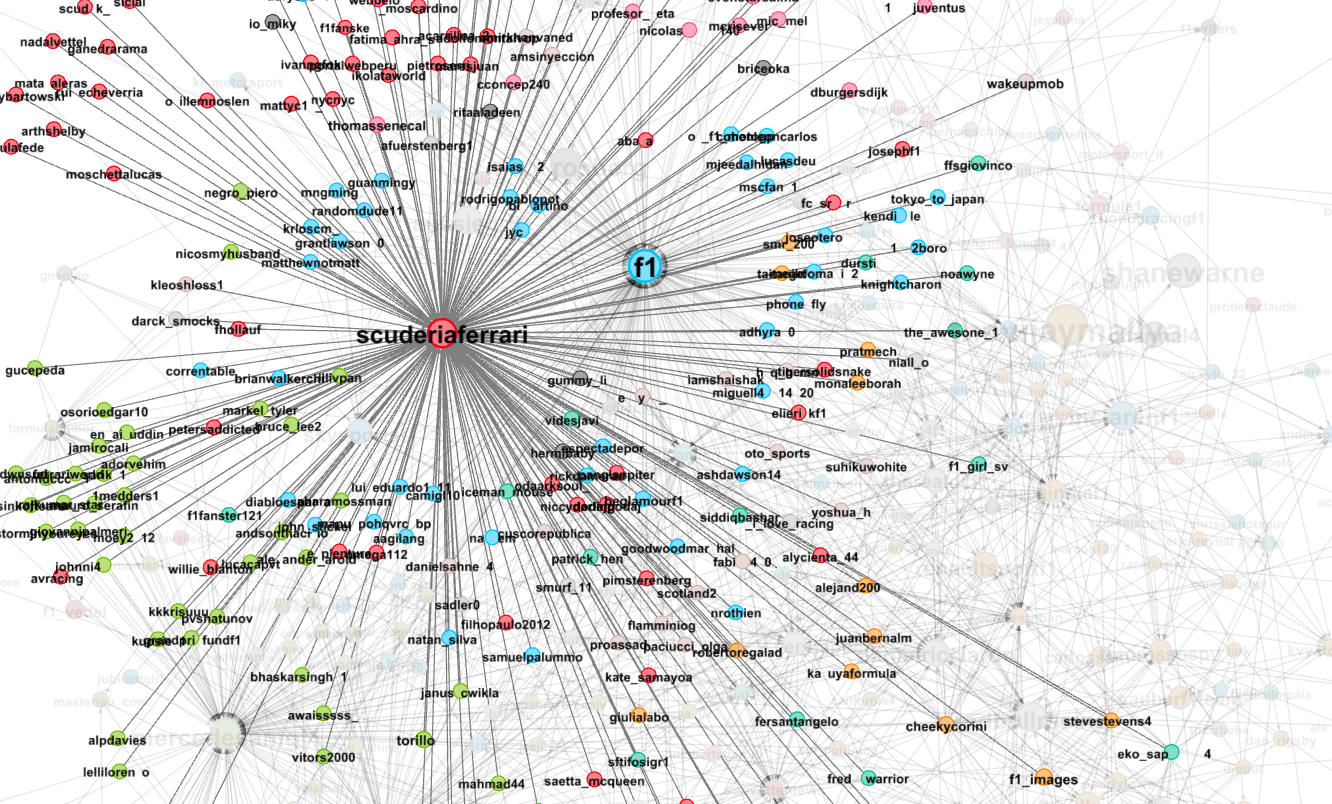
\includegraphics[width=12cm]{img/scuderiaferrari-mentions}
	\caption{Usuarios que mencionan a la cuenta @scuderiaferrari}
	\label{fig:scuderiaferrari-mentions}
\end{figure}

\begin{itemize}	
	\item \textit{@mercedesamgf1}, \textit{@lewishamilton} y \textit{@valtteribottas}: Los grandes derrotados. Un fallo en la estrategia del equipo privó de la victoria a Hamilton. Son también mencionados por todas las comunidades, pero en una proporción mucho menor a las dos cuentas anteriores (Figuras \ref{fig:mercedesamgf1-mentions}, \ref{fig:lewishamilton-mentions} y \ref{fig:valtteribottas-mentions}).
\end{itemize}

\begin{figure}[H]
	\centering
	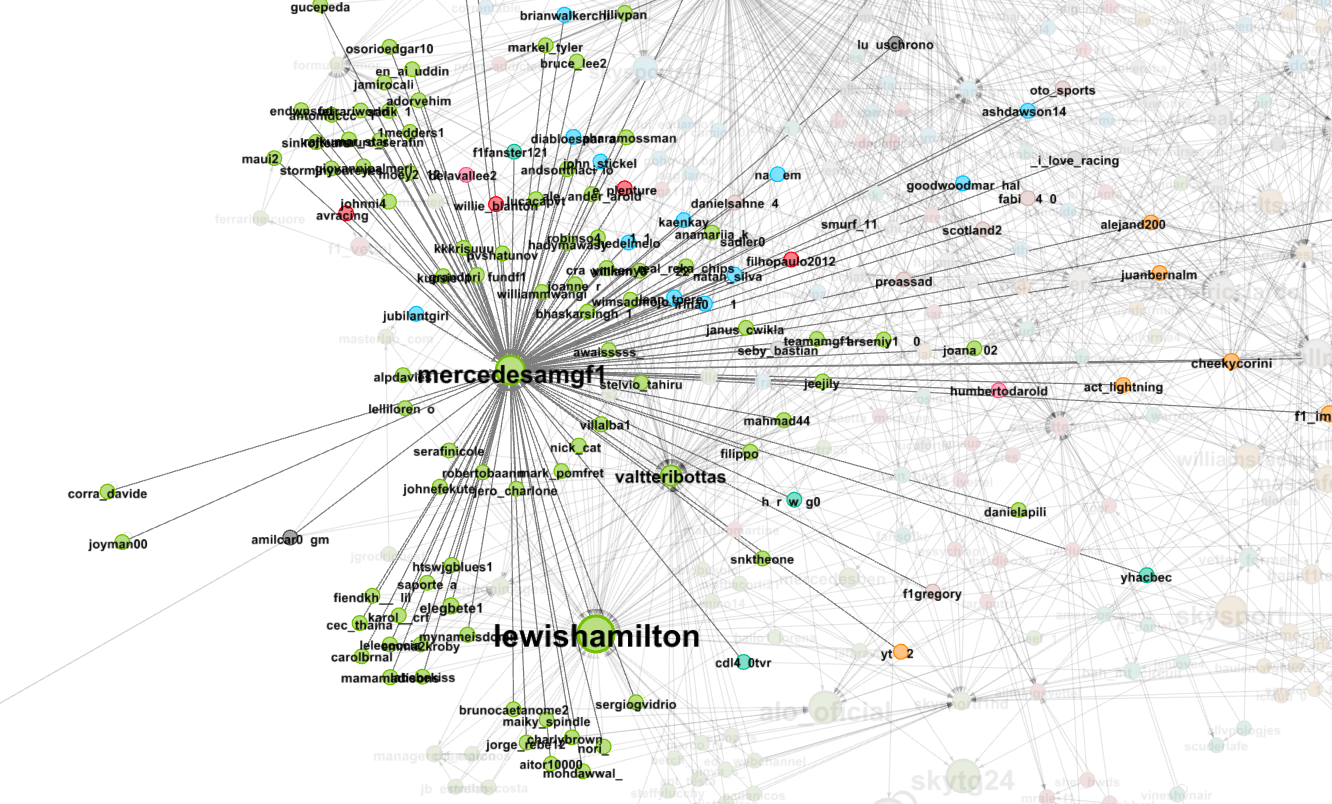
\includegraphics[width=10cm]{img/mercedesamgf1-mentions}
	\caption{Usuarios que mencionan a la cuenta @mercedesamgf1}
	\label{fig:mercedesamgf1-mentions}
\end{figure}

\begin{figure}[H]
	\centering
	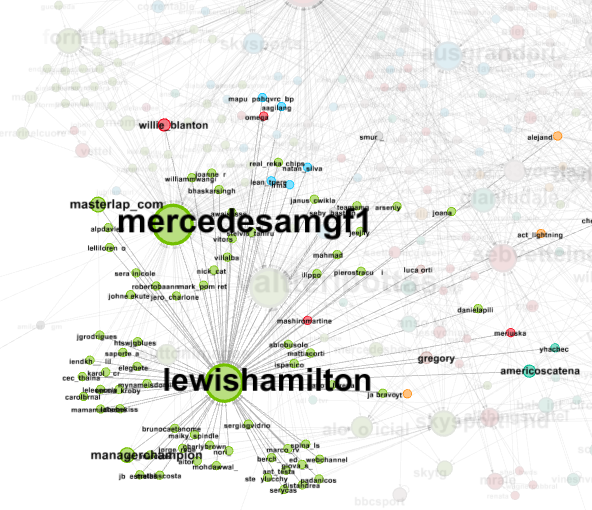
\includegraphics[width=10cm]{img/lewishamilton-mentions}
	\caption{Usuarios que mencionan a la cuenta @lewishamilton}
	\label{fig:lewishamilton-mentions}
\end{figure}

\begin{figure}[H]
	\centering
	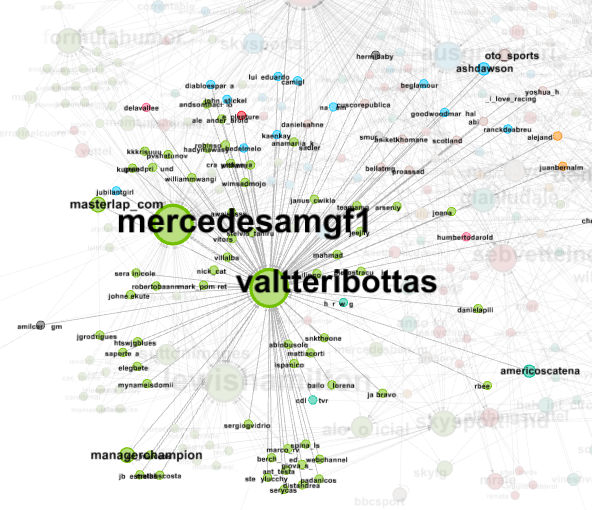
\includegraphics[width=10cm]{img/valtteribottas-mentions}
	\caption{Usuarios que mencionan a la cuenta @valtteribottas}
	\label{fig:valtteribottas-mentions}
\end{figure}

\begin{itemize}	
	\item \textit{@sebvettelnews}: A falta de cuenta oficial del piloto vencedor de la carrera, la cuenta más exitosa que publica noticias sobre él gana protagonismo.
	\item \textit{@ausgrandprix}: La cuenta oficial del Gran Premio de Australia. Se celebró allí y obviamente es muy mencionada pero no tanto como la propia cuenta oficial de la Fórmula 1.
	\item Cuentas de pilotos y equipos: En especial pilotos que tuvieron protagonismo durante la carrera, ya que otros, como Felipe Massa que, pese a lograr una buena posición, tuvo una carrera aburrida con pocas batallas en pista muestra un verde más pálido que equipos como Red Bull, Force India, Toro Rosso o McLaren y sus pilotos que animaron más la carrera.
\end{itemize}

\section{Resultados}

\subsection{Resultados obtenidos}

Una vez analizada la red social, volvemos a hacernos la pregunta que se planteó en la Sección \ref{sec:intro}: \textit{¿Qué tipo de aficionado es el mayoritario, el neutral que menciona a más de un piloto o escudería o el fanático que solo menciona a un piloto o escudería?}
\\ \\
Si primasen los usuarios fanáticos habríamos encontrado comunidades alrededor de cada piloto, sin embargo, solo encontramos una alrededor de Checo Pérez. Además, vimos como el nodo con mayor grado de entrada es el de la cuenta oficial de la escudería Ferrari, la cuál ganó la carrera. Esto nos hace pensar que los aficionados, mayoritariamente no son fanáticos de un único piloto, o al menos no lo demuestran en las redes sociales.
\\ \\
Cuando se analizaron los actores principales nos aparecieron los siguientes cuando se usaba el vector propio:

\begin{itemize}
	\item \textit{@scuderiaferrari}: Principal protagonista de la carrera.
	\item \textit{@f1}: Cuenta oficial de la Fórmula 1.
	\item \textit{@mercedesamgf1}: La escudería favorita para que uno de sus pilotos ganase la carrera y acabó derrotada obteniendo un segundo y tercer puesto para sus pilotos que supo a poco.
	\item \textit{@valteribottas}: Debutó con Mercedes e hizo una carrera sólida donde no pudo pasar del tercer puesto.
	\item \textit{@lewishamilton}: Perdió la carrera por culpa de un error de su equipo.
	\item \textit{@oconesteban}: En su debut a los volantes de un Force India logró acabar entre los diez primeros.
	\item \textit{@ausgrandprix}: Cuenta oficial del Gran Premio de Fórmula 1 de Australia.
	\item \textit{@sebvettelnews}: Cuenta que publica noticias sobre Sebastian Vettel, el cual ganó la carrera y, al no tener cuenta oficial, esta cuenta se vio beneficiada llevándose muchas menciones dirigidas hacia el piloto alemán.
	\item \textit{@danielricciardo}: No logró acabar la carrera lo que supuso una decepción, pues aspiraba al podio.
	\item \textit{@redbullracing}: Se esperaba que fuesen los principales rivales de Mercedes, pero se vieron superados por Ferrari en este primer asalto de la temporada.
\end{itemize}

Como podemos ver, los pilotos y escuderías que hay entre los diez actores principales coinciden con los principales protagonistas de la carrera lo cual responde a la segunda parte de la pregunta que se lanzó en la Sección \ref{sec:intro}: \textit{¿coincidirán los actores principales con los protagonistas de la carrera?}

\subsection{Comparación con otras redes sociales}

Las redes sociales que hemos visto en clase son:

\begin{itemize}
	\item Compañeras de mesa residencia femenina
	\item Club de kárate de Zachary
	\item Primera temporada de juego de tronos
	\item Elecciones generales 20D 2015
\end{itemize}

Por lo que lo primero que se va a hacer es una tabla (Tabla \ref{tab:comparacion-medidas}) con sus valores de medidas como se hizo para nuestra red en la Sección \ref{sec:medidas}:

\begin{table}[H]
	\centering
	\caption{Comparativa de valores de las medidas de análisis de nuestra red social con las vistas en clase}
	\label{tab:comparacion-medidas}
	\begin{tabular}{| l | l l l l l|}
		\hline
		Medida    & AusGP & Dining & Zachary & T1 JdT & 20D 2015 \\ 
		\hline
		Dirigido  & Sí    & Sí     & No      & No     & Sí       \\
		$N$       & 532   & 26     & 34      & 120    & 1807     \\
		$L$       & 1783  & 52     & 78      & 317    & 8639     \\
		$D$       & 0,006 & 0,08   & 0,139   & 0,044  & 0,003    \\
		$k$       & 3,352 & 2      & 2,294   & 5,283  & 4,781    \\
		$d_{max}$ & 4     & 7      & 3       & 7      & 18       \\
		$d$       & 1,189 & 2,839  & 1,274   & 3,307  & 5,386    \\
		$C$       & 0,131 & 0,069  & 0,285   & 0,604  & 0,293    \\
		\hline
	\end{tabular}
\end{table}

En cuanto a tamaño de red no hay ninguna que se le asemeje. Las primeras al ser de grupos sociales cerrados tienen un tamaño muy reducido, y la de las elecciones contiene muchos más tuits que los que yo pude recopilar. No obstante, al ser ambas extraidas de twitter tienen en común la baja densidad, aún menor en la de las elecciones que en la nuestra.
\\ \\
En cuanto a grado, la más parecida es la de las elecciones (un grado algo mayor) y la del club de kárate (un grado algo menor).
\\ \\
En distancia media y diámetro la que más se asemeja es la del club de kárate y en coeficiente de clustering se vuelven a repetir las de las elecciones y la de kárate como las más parecidas.
\\ \\
Por tanto vemos que las más parecidas son tanto la de las elecciones, que en lo que más difiere es en las distancias y la de kárate que difiere bastante en la topología de la red ya que es mucho más pequeña y no es dirigida.

%----------------------------------------------------------------------------------------
%	REFERENCIAS
%----------------------------------------------------------------------------------------

\newpage

%\bibliography{referencias} %archivo referencias.bib que contiene las entradas 
%\bibliographystyle{plain} % hay varias formas de citar

\end{document}